%
%===============>>  Ленотьева Модуль 6 <<=============
%
\setmodule{7}

%BEGIN_FOLD % ====>>_____ Занятие 1 _____<<====
\begin{class}[number=1]
	\begin{listofex}
		\item На рисунке изображён график функции \( y=f(x) \) левая круглая скобка x правая круглая скобка . Какие из утверждений относительно этой функции неверны? Укажите их номера.
		\begin{figure}[h!]
			\centering
			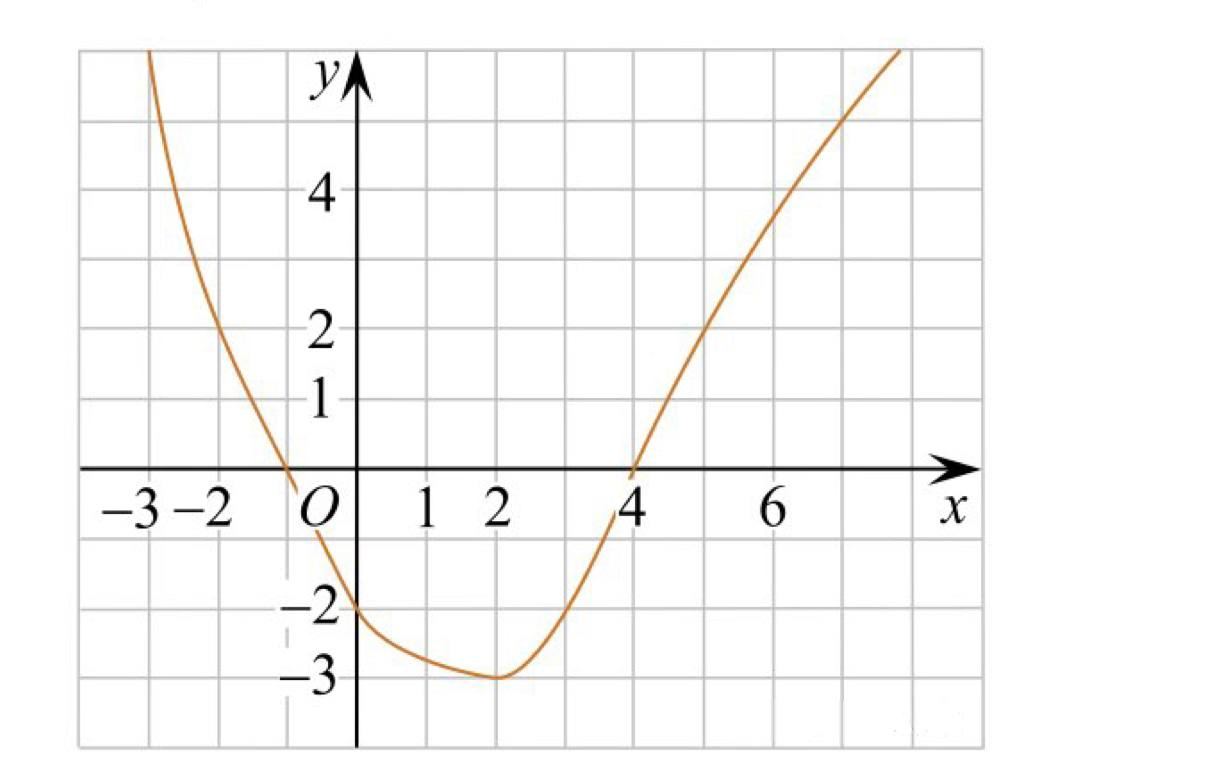
\includegraphics[width=0.7\linewidth]{../../../../../exercises/lists/pics/leontevaM7L2-1}
		\end{figure}
		\begin{tasks}(1)
			\task функция возрастает на промежутке  \( [-2; +\infty) \)
			\task \( f(3)> f(-3)  \)
			\task \( f(0) = -2 \)
			\task прямая y=2  пересекает график в точках \(  (-2; 2) \)  и \( (5; 2) \) 
		\end{tasks}
	\newpage
		\item На рисунке изображён график квадратичной функции \( y  =  f(x) \).
		\\
		Какие из следующих утверждений о данной функции неверны? Запишите их номера в порядке возрастания.
		\begin{figure}[h!]
			\centering
			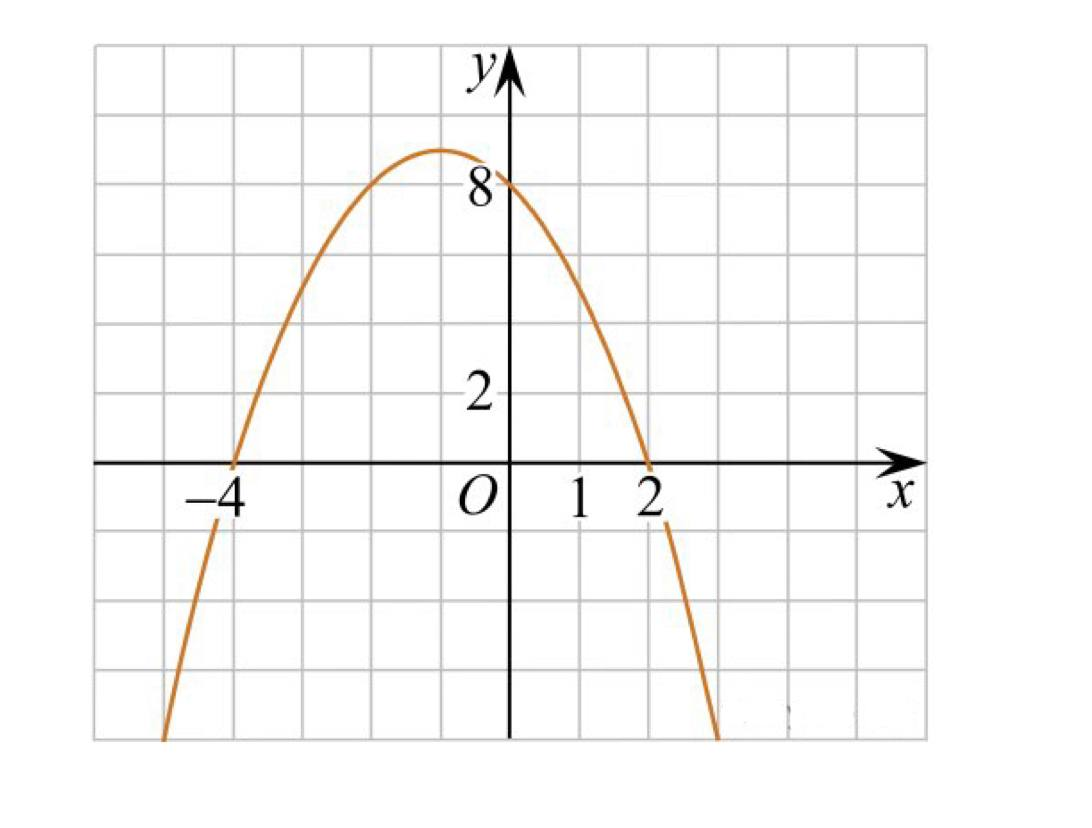
\includegraphics[width=0.7\linewidth]{../../../../../exercises/lists/pics/leontevaM7L2-2}
		\end{figure}
		\begin{tasks}(1)
			\task Функция возрастает на промежутке \( (-\infty;  -1 \)].
			\task Наибольшее значение функции равно \( 8 \).
			\task \( f(-4) \neq f(2) \).
		\end{tasks}
	\newpage
	\item На рисунке изображён график квадратичной функции \( y =  f(x) \).
	Какие из следующих утверждений о данной функции неверны? Запишите их номера.
	\begin{figure}[h!]
		\centering
		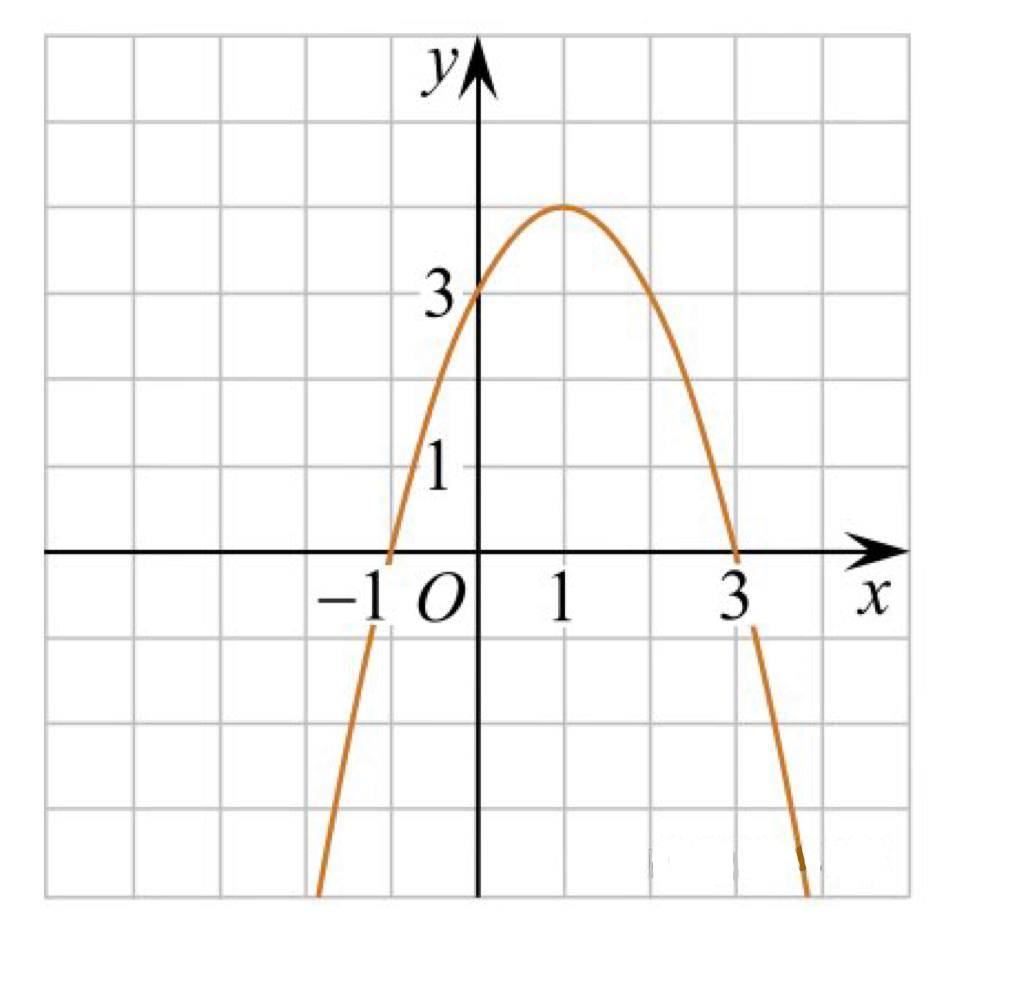
\includegraphics[width=0.7\linewidth]{../../../../../exercises/lists/pics/leontevaM7L2-3}
	\end{figure}
	\begin{tasks}(1)
		\task \( f(-1)=f(3) \).
		\task Наибольшее значение функции равно \( 3 \).
		\task \( f(x)>0  \) при  \( -1<x<3 \).
	\end{tasks}
	\newpage
	\item На рисунке изображён график квадратичной функции \( y = f(x) \).
	
	Какие из следующих утверждений о данной функции неверны? Запишите их номера.
	\begin{figure}[h!]
		\centering
		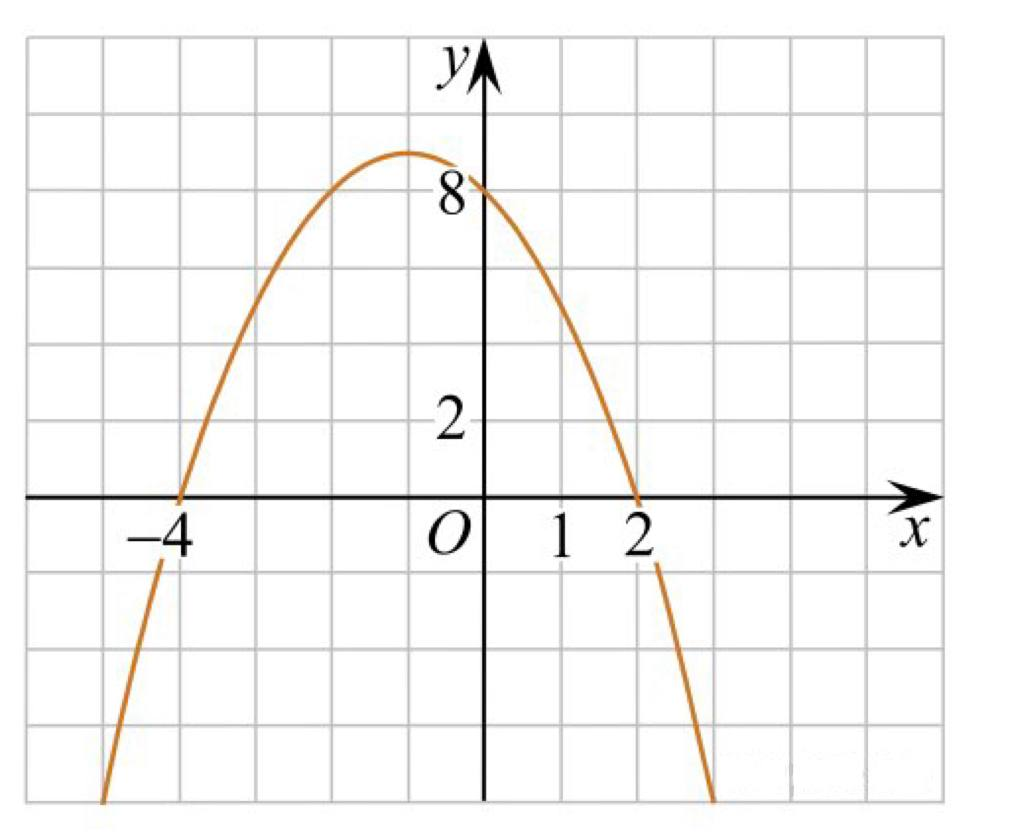
\includegraphics[width=0.7\linewidth]{../../../../../exercises/lists/pics/leontevaM7L2-4}
	\end{figure}
	\begin{tasks}(1)
		\task  Наибольшее значение функции равно \( 9 \).
		\task \( f(0)>f(1) \).
		\task \( f( x )>0 \) при \( x<0 \).
	\end{tasks}
	\newpage
	\item На рисунке изображён график функции\(  y = ax2 + bx + c \). Установите соответствие между утверждениями и промежутками, на которых эти утверждения выполняются. 
	\begin{figure}[h!]
		\centering
		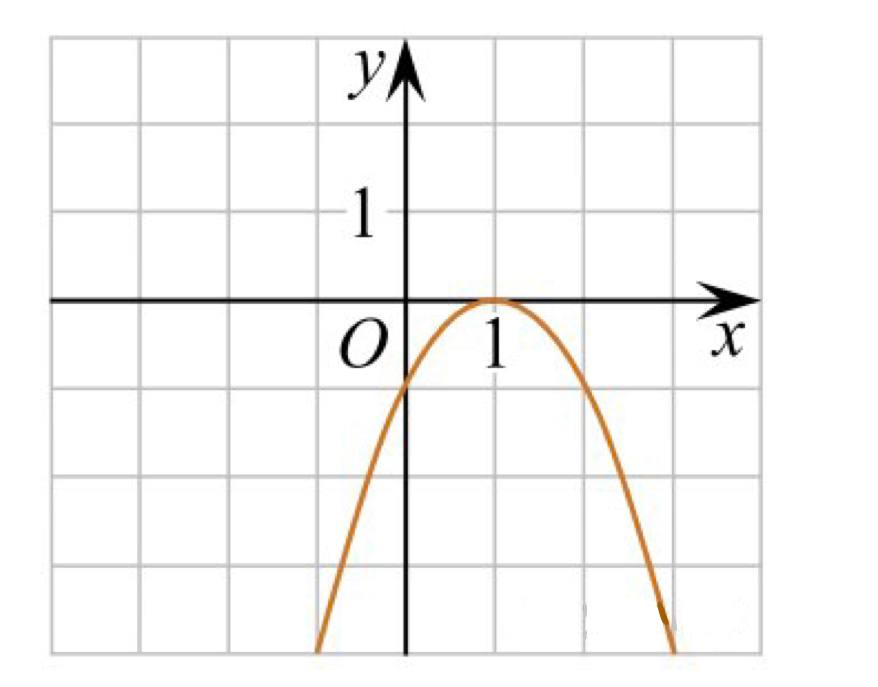
\includegraphics[width=0.7\linewidth]{../../../../../exercises/lists/pics/leontevaM7L2-5}
	\end{figure}
	\begin{tasks}(2)
		\task[] УТВЕРЖДЕНИЯ	 
		\task[]	ПРОМЕЖУТКИ
		\task[A)] функция возрастает на промежутке
		\task \( [1;2] \)
		\task[B)]функция убывает на промежутке
		\task \( [0;2] \)
		\task[]
		\task\( [-1;0] \)
		\task[]
		\task\( [-2;3] \)
	\end{tasks}
	\newpage
	\item 
	На рисунке изображён график функции\(  y = ax2 + bx + c \). Установите соответствие между утверждениями и промежутками, на которых эти утверждения выполняются. 
	\begin{figure}[h!]
		\centering
		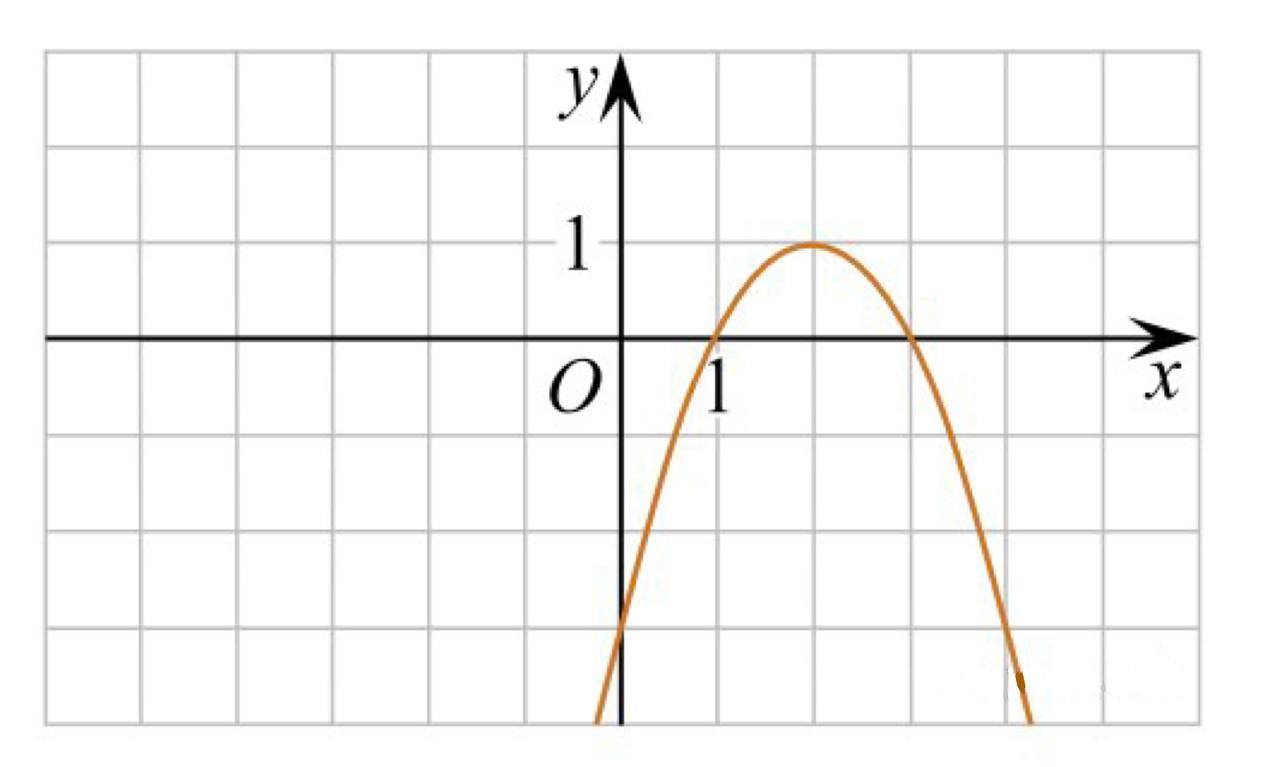
\includegraphics[width=0.7\linewidth]{../../../../../exercises/lists/pics/leontevaM7L2-6}
	\end{figure}
	\begin{tasks}(2)
		\task[] УТВЕРЖДЕНИЯ	 
		\task[]	ПРОМЕЖУТКИ
		\task[A)] функция возрастает на промежутке
		\task \( [0; 3] \)
		\task[B)]функция убывает на промежутке
		\task \( [-1; 1] \)
		\task[]
		\task\( [2; 4] \)
		\task[]
		\task\( [1; 4] \)
	\end{tasks}
	\item Найдите координаты вершины параболы \( у = 2x^{2} + 4x + 5 \).
	\item Найдите координаты вершины параболы\(  у = -x^{2} + 2x - 4 \).
	\item Найдите координаты вершины параболы\(  у = \dfrac{1}{3}x^{2}+x-1 \).
	\item Найти вершину параболы, заданной формулой \( y=2x^{2} - 8x + 5. \)
	\item Парабола проходит через точки \( K(0; –5) \), \( L(3; 10) \), \(  M( –3; –2) \). Найдите координаты её вершины.
	\item Парабола проходит через точки \(  K(0; –2) \), \(  L(4; 6) \), \( M(1; 3) \). Найдите координаты её вершины.
	\item Парабола проходит через точки \( A(0; 4) \), \( B(1; 11) \), \( C(–5; –1) \). Найдите координаты её вершины.
	\item При каких значениях \(  p \) вершины парабол \( y=-x^{2}+2px+3 \) и \\\ \( y=x^{2}-6px+p \) расположены по разные стороны от оси \( x \) ?
	\item Решите систему неравенств  
	\begin{equation*}
		\begin{cases}
			7(3x+2)-3(7x+2)>2x
			\\
			(x-5)(x+8)<0
		\end{cases}
	\end{equation*}
	\item Решите систему неравенств  
	\begin{equation*}
		\begin{cases}
			\dfrac{10-2x}{3+(5-2x)^{2}\geq0}
			\\
			2-7x\leq14-3x
		\end{cases}
	\end{equation*}
	\item Решите систему неравенств  
	\begin{equation*}
		\begin{cases}
			4(9x+3)-9(4x+3)>3x
			\\
			(x-2)(x+9)<0
		\end{cases}
	\end{equation*}
	\end{listofex}
	
\end{class}
%END_FOLD

%BEGIN_FOLD % ====>>_____ Занятие 2 _____<<====
\begin{class}[number=2]
	\begin{listofex}
		\item Занятие 2
	\end{listofex}
\end{class}
%END_FOLD

%BEGIN_FOLD % ====>>_ Домашняя работа 1 _<<====
\begin{homework}[number=1]
	\begin{listofex}
		\item Домашняя работа 1
	\end{listofex}
\end{homework}
%END_FOLD

%BEGIN_FOLD % ====>>_____ Занятие 3 _____<<====
\begin{class}[number=3]
	\begin{listofex}
		\item Занятие 3 
	\end{listofex}
\end{class}
%END_FOLD

%BEGIN_FOLD % ====>>_____ Занятие 4 _____<<====
\begin{class}[number=4]
	\begin{listofex}
		\item Занятие 4
	\end{listofex}
\end{class}
%END_FOLD

%BEGIN_FOLD % ====>>_ Домашняя работа 2 _<<====
\begin{homework}[number=2]
	\begin{listofex}
		\item Домашняя работа 2
	\end{listofex}
\end{homework}
%END_FOLD

%BEGIN_FOLD % ====>>_____ Занятие 5 _____<<====
\begin{class}[number=5]
	\begin{listofex}
		\item Занятие 5
	\end{listofex}
\end{class}
%END_FOLD

%BEGIN_FOLD % ====>>_____ Занятие 6 _____<<====
\begin{class}[number=6]
	\begin{listofex}
		\item Занятие 6
	\end{listofex}
\end{class}
%END_FOLD

%BEGIN_FOLD % ====>>_ Домашняя работа 3 _<<====
\begin{homework}[number=3]
	\begin{listofex}
		\item Домашняя работа 3
	\end{listofex}
\end{homework}
%END_FOLD

%BEGIN_FOLD % ====>>_____ Занятие 7 _____<<====
\begin{class}[number=7]
	\title{Подготовка к проверочной}
	\begin{listofex}
		\item Занятие 7
	\end{listofex}
\end{class}
%END_FOLD

%BEGIN_FOLD % ====>>_ Проверочная работа _<<====
\begin{exam}
	\begin{listofex}
		\item Проверочная
	\end{listofex}
\end{exam}
%END_FOLD